\documentclass[aspectratio=169, xcolor=dvipsnames]{beamer}

% --- Theme Setup ---
\usetheme{Madrid}
\usecolortheme{default}

% --- Packages ---
\usepackage{graphicx}
\usepackage{xcolor}
\usepackage{booktabs}
\usepackage{hyperref}
\usepackage{adjustbox}
\usepackage{amssymb}
\usepackage{amsmath}
\usepackage{longtable}
\usepackage{caption}

% --- Title Information ---
\title{Module 07}
\subtitle{Introduction to Relational Model/2}
\author{Milav Dabgar}
\institute{www.milav.in}
\date{\today}

\begin{document}

% Title Slide
\begin{frame}
    \titlepage
\end{frame}

\begin{frame}{Module Recap}
    \begin{itemize}[<+->]
        \item Basic notions of modeling introduced
        \item Attributes and their Types
        \item Schema and Instance
        \item Keys and their Categorization
        \item Languages for Relation Model introduced
    \end{itemize}
\end{frame}

\begin{frame}{Module Objectives}
    \begin{block}{Goals}
        \begin{itemize}[<+->]
            \item To understand relational algebra
            \item To familiarize with the operators of relational algebra
        \end{itemize}
    \end{block}
\end{frame}

\begin{frame}{Module Outline}
    \begin{itemize}[<+->]
        \item \textbf{Operations}
        \begin{itemize}
            \item Select
            \item Project
            \item Union
            \item Difference
            \item Intersection
            \item Cartesian Product
            \item Natural Join
        \end{itemize}
        \item \textbf{Aggregate Operations}
    \end{itemize}
\end{frame}

\section{Relational Operators}

\begin{frame}
  \vfill
  \centering
  \begin{beamercolorbox}[sep=8pt,center,shadow=true,rounded=true]{title}
    \usebeamerfont{title}Relational Operators\par%
  \end{beamercolorbox}
  \vfill
\end{frame}

\begin{frame}{Basic Properties of Relations}
    \begin{block}{A relation is a set. Hence,}
        \begin{itemize}[<+->]
            \item \textbf{Ordering of rows / tuples is inconsequential}
        \end{itemize}
        \begin{center}
            \begin{tabular}{|l|l|}
            \hline
            \textbf{A} & \textbf{B} \\ \hline
            a1 & b1 \\ \hline
            a1 & b2 \\ \hline
            a2 & b1 \\ \hline
            a2 & b2 \\ \hline
            \end{tabular}
            \quad \textit{is same as:} \quad
            \begin{tabular}{|l|l|}
            \hline
            \textbf{A} & \textbf{B} \\ \hline
            a1 & b1 \\ \hline
            a2 & b1 \\ \hline
            a2 & b2 \\ \hline
            a1 & b2 \\ \hline
            \end{tabular}
        \end{center}
    \end{block}
    
    \uncover<2->{
        \begin{alertblock}{All rows / tuples must be distinct}
            \begin{center}
                \begin{tabular}{|l|l|}
                \hline
                \textbf{A} & \textbf{B} \\ \hline
                a1 & b1 \\ \hline
                a1 & b2 \\ \hline
                a1 & b2 \\ \hline
                a1 & b1 \\ \hline
                \end{tabular}
                \quad \textit{is not valid}
            \end{center}
        \end{alertblock}
    }
\end{frame}

\begin{frame}{Select Operation - selection of rows (tuples)}
    \begin{itemize}
        \item Relation $r$
        \item $\sigma_{A=B \wedge D>5}(r)$
    \end{itemize}
    \begin{center}
        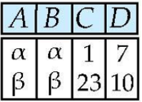
\includegraphics[height=0.6\textheight, width=\textwidth, keepaspectratio]{../Lecture 2.2_artifacts/image_000007_5bbbab4ed5988d9e24e35c2bbc52c80ff2e35316200ed543c7f176a7956c9e39.png}
    \end{center}
\end{frame}

\begin{frame}{Project Operation - selection of columns (Attributes)}
    \begin{itemize}
        \item Relation $r$
        \item $\pi_{A,C}(r)$
    \end{itemize}
    \begin{center}
        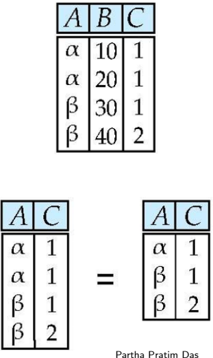
\includegraphics[height=0.6\textheight, width=\textwidth, keepaspectratio]{../Lecture 2.2_artifacts/image_000009_ef40dbcd1acaa14719c70cb972cfcd6b7251322f75d269e4d9d0e9d379bdc4af.png}
    \end{center}
\end{frame}

\begin{frame}{Union of two relations}
    \begin{itemize}
        \item Relation $r, s$
        \item $r \cup s$
    \end{itemize}
    \begin{center}
        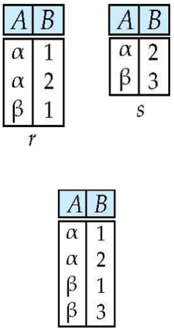
\includegraphics[height=0.6\textheight, width=\textwidth, keepaspectratio]{../Lecture 2.2_artifacts/image_000011_ce3c882bf595af49413e64554f8e692b0660ac980729f9fd01fc3b81af84eabc.png}
    \end{center}
\end{frame}

\begin{frame}{Set difference of two relations}
    \begin{itemize}
        \item Relation $r, s$
        \item $r - s$
    \end{itemize}
    \begin{center}
        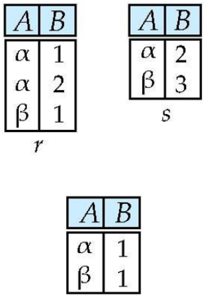
\includegraphics[height=0.6\textheight, width=\textwidth, keepaspectratio]{../Lecture 2.2_artifacts/image_000013_32ed706f37d3f77c48bdc975c14057082a5f70e984274b910b15cf6fe87b52fa.png}
    \end{center}
\end{frame}

\begin{frame}{Set intersection of two relations}
    \begin{itemize}
        \item Relation $r, s$
        \item $r \cap s$
        \item \textbf{Note:} $r \cap s = r - (r - s)$
    \end{itemize}
    \begin{center}
        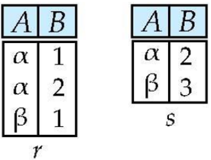
\includegraphics[height=0.5\textheight, width=\textwidth, keepaspectratio]{../Lecture 2.2_artifacts/image_000015_04bf9ac366dd968ba53eae566267cab1d15aaeedac1fbc52dc8be7b3c89ca01a.png}
    \end{center}
\end{frame}

\begin{frame}{Joining two relations - Cartesian-product}
    \begin{itemize}
        \item Relation $r, s$
        \item $r \times s$
    \end{itemize}
    \begin{center}
        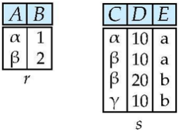
\includegraphics[height=0.35\textheight, width=\textwidth, keepaspectratio]{../Lecture 2.2_artifacts/image_000018_a0176a3313262ecd1e9727a86ddb08333c0ec42f560f01141d35b77826a18d31.png}
        \vspace{0.5em}
        
        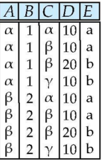
\includegraphics[height=0.35\textheight, width=\textwidth, keepaspectratio]{../Lecture 2.2_artifacts/image_000019_b277e58487b771d787ee36eb0221179f9d51ada48639e6bf8c4c7c48de92009b.png}
    \end{center}
\end{frame}

\begin{frame}{Cartesian-product - naming issue}
    \begin{itemize}
        \item Relation $r, s$
        \item $r \times s$
    \end{itemize}
    \begin{center}
        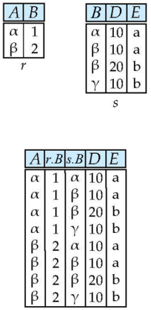
\includegraphics[height=0.6\textheight, width=\textwidth, keepaspectratio]{../Lecture 2.2_artifacts/image_000021_c73eaa300396c98eb55b9d3b095f52f96b9fc31a7a8ab837d64fad7590978c98.png}
    \end{center}
\end{frame}

\begin{frame}{Renaming a Table}
    \begin{itemize}
        \item Allows us to refer to a relation, (say $E$) by more than one name.
        \item $\rho_X(E)$ : returns the expression $E$ under the name $X$
        \item Relations $r$
        \item $r \times \rho_s(r)$
    \end{itemize}
    \begin{center}
        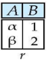
\includegraphics[height=0.25\textheight, width=\textwidth, keepaspectratio]{../Lecture 2.2_artifacts/image_000023_66d8a128dead735d13b126ab41f2f705e07fc2d88c78a5598f3565df723660a6.png}
        \vspace{0.5em}
        
        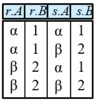
\includegraphics[height=0.25\textheight, width=\textwidth, keepaspectratio]{../Lecture 2.2_artifacts/image_000024_720123ba8fc85f8bba37b5663ae12cf72bfeebcf36a00f1cf3af6dcb0e144a13.png}
    \end{center}
\end{frame}

\begin{frame}{Composition of Operations}
    \begin{itemize}
        \item Can build expressions using multiple operations
        \item Example: $\sigma_{A=C}(r \times s)$
        \item $r \times s$
        \item $\sigma_{A=C}(r \times s)$
    \end{itemize}
    \begin{center}
        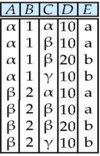
\includegraphics[height=0.45\textheight, width=\textwidth, keepaspectratio]{../Lecture 2.2_artifacts/image_000026_23455047d65674637cb49ce6e93c50ef3a92b6858608443a823a4a4c62b5b976.png}
    \end{center}
\end{frame}

\begin{frame}{Joining two relations - Natural Join}
    \begin{block}{Definition}
        \begin{itemize}[<+->]
            \item Let $r$ and $s$ be relations on schemas $R$ and $S$ respectively. Then, the \textbf{natural join} of relations $R$ and $S$ is a relation on schema $R \cup S$ obtained as follows:
            \item Consider each pair of tuples $t_r$ from $r$ and $t_s$ from $s$.
            \item If $t_r$ and $t_s$ have the same value on each of the attributes in $R \cap S$, add a tuple $t$ to the result, where
            \begin{itemize}
                \item[$\triangleright$] $t$ has the same value as $t_r$ on $r$
                \item[$\triangleright$] $t$ has the same value as $t_s$ on $s$
            \end{itemize}
        \end{itemize}
    \end{block}
\end{frame}

\begin{frame}{Natural Join Example}
    \begin{itemize}
        \item Relations $r, s$:
        \item Natural Join
        \item[] $r \bowtie s = \pi_{A, r.B, C, r.D, E}(\sigma_{r.B = s.B \wedge r.D = s.D}(r \times s))$
    \end{itemize}
    \begin{center}
        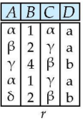
\includegraphics[height=0.3\textheight, width=\textwidth, keepaspectratio]{../Lecture 2.2_artifacts/image_000030_14420a552c73d01aa3cfe279ebe7805a78819bd21daae47055aa0f6d6fabfe86.png}
        \vspace{0.2em}
        
        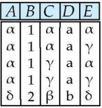
\includegraphics[height=0.3\textheight, width=\textwidth, keepaspectratio]{../Lecture 2.2_artifacts/image_000032_35687e3f5ebada05f6fa62971d6dc0630bd5fb3952a7f7a0c2a6e1b466d30538.png}
    \end{center}
\end{frame}

\section{Aggregation Operators}

\begin{frame}
  \vfill
  \centering
  \begin{beamercolorbox}[sep=8pt,center,shadow=true,rounded=true]{title}
    \usebeamerfont{title}Aggregation Operators\par%
  \end{beamercolorbox}
  \vfill
\end{frame}

\begin{frame}{Aggregate Operators}
    \begin{exampleblock}{Common Functions}
        \begin{itemize}[<+->]
            \item Can we compute:
            \begin{itemize}
                \item \textbf{SUM}
                \item \textbf{AVG}
                \item \textbf{MAX}
                \item \textbf{MIN}
            \end{itemize}
        \end{itemize}
    \end{exampleblock}
\end{frame}

\begin{frame}{Notes about Relational Languages}
    \begin{itemize}
        \item Each query input is a table (or set of tables)
        \item Each query output is a table
        \item All data in the output table appears in one of the input tables
        \item Relational Algebra is \textbf{not} Turing complete
    \end{itemize}
\end{frame}

\begin{frame}{Summary of Relational Algebra Operators}
    \begin{center}
        \begin{adjustbox}{max width=\textwidth}
        \begin{tabular}{lll}
        \toprule
        \textbf{Symbol} (Name) & \textbf{Example of Use} & \textbf{Description} \\ \midrule
        $\sigma$ (Selection) & $\sigma_{\text{salary} \ge 85000}(\text{instructor})$ & Return rows of the input relation that satisfy the predicate. \\
        $\pi$ (Projection) & $\pi_{\text{ID}, \text{salary}}(\text{instructor})$ & Output specified attributes from all rows ... Remove duplicates. \\
        $\times$ (Cartesian Product) & $\text{instructor} \times \text{department}$ & Output all possible combinations of rows from the two relations. \\
        $\cup$ (Union) & $\pi_{name}(\text{student}) \cup \pi_{name}(\text{instructor})$ & Output the union of tuples from the two input relations. \\
        $-$ (Set Difference) & $\pi_{name}(\text{student}) - \pi_{name}(\text{instructor})$ & Output the set difference of tuples. \\
        $\bowtie$ (Natural Join) & $\text{instructor} \bowtie \text{department}$ & Output pairs of rows that agree on values of common attributes. \\
        \bottomrule
        \end{tabular}
        \end{adjustbox}
    \end{center}
\end{frame}

\begin{frame}{Module Summary}
    \begin{itemize}
        \item Introduced relational algebra
        \item Familiarized with the operators of relational algebra
    \end{itemize}
    \vspace{2em}
    \begin{center}
    \small \textit{Slides used in this presentation are borrowed from \url{http://db-book.com/} with kind permission of the authors.} \\
    \small \textit{Edited and new slides are marked with 'PPD'.}
    \end{center}
\end{frame}

\end{document}
